\section{Workload Generation}
\label{se:workload}

As explained in Chapter \ref{ch:method}, timeseries has six primary attributes. To create a timeseries for performance testing, it needs data for each key attribute.
While generating the timeseries for performance testing, it selected locations all over the world as a generic case to include all the locations without binding to a specific area.

These locations are taken from Google's Countries Public Data set \cite{GoogleGoogleCounties}, and consider static though out the testing, and data added to the wdias-performance-test.
During the performance test, it creates 1000 timeseries and keeps adding data against those timeseries. For each location, it creates four timeseries \hl{as a combination of four values of moduleId key attribute}. Thus combining all together, those create 1000 timeseries. But test cases generate these values before starts the performance tests, and able to increase the timeseries as wanted.

For grid data, it uses static 100 grid locations based on how is \acrshort{api} exposed. Since grid locations have different metadata structures as described in \cref{se:db_struct}, those data handle separately. But the locationId of grid and scalar data types have the same effect when defining a timeseries.

In the  JMeter Best Practices, \say{If your test needs large amounts of data - particularly if it needs to be \emph{randomized} create the test data in a file that can be read with CSV Data set. This avoids wasting resources at run-time}. Rather providing the randomness in run time, the timeseries stored with the random order which satisfy the percentage of 70\% Scalar, 20\% Vector, and 10\% Grid as mentioned in \cref{se:test_plan}.
Before running the test cases, it generates the metadata for timeseries and writes into a CSV file which is shared among the threads in the  JMeter. This occurs in the setup phase of the test cases. The metadata CSV file arrange in a way that within every 10 lines, 7 lines are Scalar timeseries, 2 lines are Vector timeseries, and 1 line is a Grid timeseries.

The system is capable of storing any numeric value up to 3 decimal points. It does not make any difference based on the parameter type whether it is the precipitation or the temperature. Thus during the performance testing,  JMeter uses real precipitation data from \acrshort{curw}. One month period of data for five weather stations has been using to prepare the test data. The script to clean up and prepare the precipitation data is available as \emph{setup\_precipitation.sh} in wdias-performance.

\begin{lstlisting}[language=sh, caption=Preparation of precipitation data.]
Set ROOT_DIR=~/wdias/wdias-performance-test
-h | --help: Usage
  setup_precipitation.sh  <COMMAND>
    - COMMAND: help | extract | prepare | cleanup | populate
  e.g.
  setup_precipitation.sh prepare
    Segregate single file data into multiple files based on date. And Separate into main directories of 15min, 30min, 60min and create tar files
  setup_precipitation.sh extract
    Extract the tar files into 15min, 30min and 60min
  setup_precipitation.sh cleanup
    Clean up extracted directories
\end{lstlisting}
When preparing the data, it creates three sets of data based on the time interval such as hourly (60min), 30min, and 15min data with modifying the replicated data.
This will reduce the overhead in performance testing and increase the performance itself.
Extract function use while creating the containers, and extract the data into the container. This reduces the context loading while creating the container images.
While performing the load testing,  JMeter keeps update a date counter and creates over the one-month data. At the end of the current month, the date counter advance to the next month. But data is repeated using from the beginning. To provide more randomness, it switches over five locations as well. The JSR223 scripts were written generically such that is possible to tweak and use if there are more location data available.

Almost similar to how was the precipitation data proceed, the water level is prepared for Grid data. The Grid data files are real data output of FLO2D 150 meter hydrology model which uses in the \acrshort{curw}. Each file follow the format of ASCII Grid file and consist of 120 rows and 139 columns with using the \texttt{-9} for the missing data as an optimization. Each file size is 50,337 Bytes (50 Kilobytes).
% One exception with Grid data during these test cases was, the maximum time step is 30min, instead of 15min due to the larger size of the data. But the \acrshort{wdias} is capable of supporting such request. The main purpose of the \acrshort{wdias} is to provide an extensible architecture framework, during the performance testing it is not much considered about scaling the Grid data handling as it using \acrshort{netCDF}, and it is another domain with an attraction up to some extent.

\begin{lstlisting}[language=sh, caption= Preparation of water-level data.]
Set ROOT_DIR=~/wdias/wdias-performance-test
-h | --help: Usage
  setup_water-level.sh  <COMMAND>
    - COMMAND: help | extract | prepare | cleanup | populate
  e.g.
  setup_water-level.sh prepare
    Segregate single file data into multiple grid file directories based on date. And Separate into main directories of 15min, 30min, 60min and create tar files
  setup_water-level.sh extract
    Extract the tar files into 15min, 30min and 60min
  setup_water-level.sh cleanup
    Clean up extracted directories
\end{lstlisting}
The water level also contains the real data for one month of period and \emph{setup\_waterlevel.sh} script provides the functionality of preparation, cleanup, and extract.
Also, it reset and repeat reading from the beginning when the  JMeter date counter keeps increasing.


%%%%%%%%%%%%%%%%%%%%%%%%%%%%%%%%%%%%%%%%%%%%%%%%%%%%%%%%%%%%%%%%%%%%%%%%%%%%%%%%
\subsection{Experimental Setup}
\label{subse:experimental_setup}

To create a higher workload using the  JMeter, it has a Distributed Testing feature. It uses the master-slave approach and it allowed to handle all the test cases via single instance, rather handling separate instances. But it has the following limitation of \emph{the same test plan runs by all the servers}.  JMeter does not distribute the load between servers, each runs the full test plan. So if you set 1,000 threads and have 6  JMeter servers, you end up injecting 6,000 threads. When test cases run with  JMeter Distributed mode, the server node trigger the same copy of the test case on configured slave nodes parallel. At the end of the test cases, it gathers results into the master node.

\begin{figure}[htp]
    \centering
    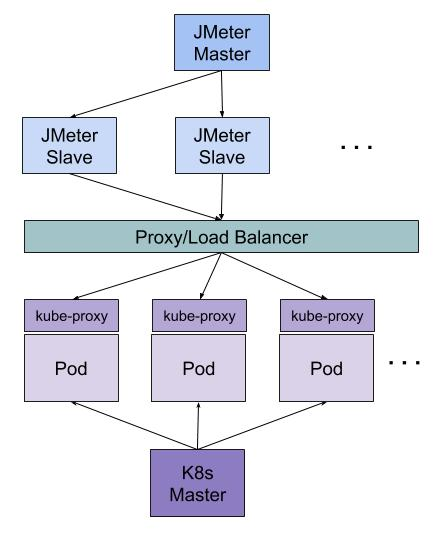
\includegraphics[width=0.6\textwidth]{results/work_load/experimental_setup_v3.jpg}
    \caption{Experimental setup with JMeter}
    \label{fi:experimental_setup}
\end{figure}

When implementing load test cases with  JMeter, it uses threads to simulate the users. The root component of a test create is a thread group. There are different kinds of thread groups are available such as thread group (basic thread group), arrivals thread Group, free form arrivals thread group, stepping thread group, concurrency thread group, and ultimate thread group.


%%%%%%%%%%%%%%%%%%%%%%%%%%%%%%%%%%%%%%%%%%%%%%%%%%%%%%%%%%%%%%%%%%%%%%%%%%%%%%%%
\subsubsection{Closed vs. open workload models}
\label{subse:closed_vs_open_workload}
\begin{itemize}
    \item \emph{closed system model} \cite{Haggett1998AnWales} -- a new request is only triggered by the completion of a previous request, following by a think time. The system has negative feedback that makes it impossible to bury-out the service, so users wait for the responses before making new requests.
    \item \emph{open system model} -- new requests arrival independently of completions, e.g., according to a stochastic process or fixed trace. The system has no negative feedback.
\end{itemize}
While implementing the test cases for \acrshort{wdias}, it uses the Concurrency Thread Group with Throughput Shaping Timer because it supports the open workload approach.
Using other thread groups, it required to find the exact number of threads and timer delays that produce the desired number of \acrfull{rps} to server. It is known as the \emph{closed workload}.
With using \emph{Throughput Shaping Timer}, it only needs to configure the \acrshort{rps}. When combining this  JMeter plugin with Concurrency Thread Group using Schedule Feedback Function to dynamically maintain thread count required to achieve target \acrshort{rps} \cite{KarunarathneGihanWdias/wdias-performance-test:JMeter.}.

\begin{figure}[htp]
    \centering
    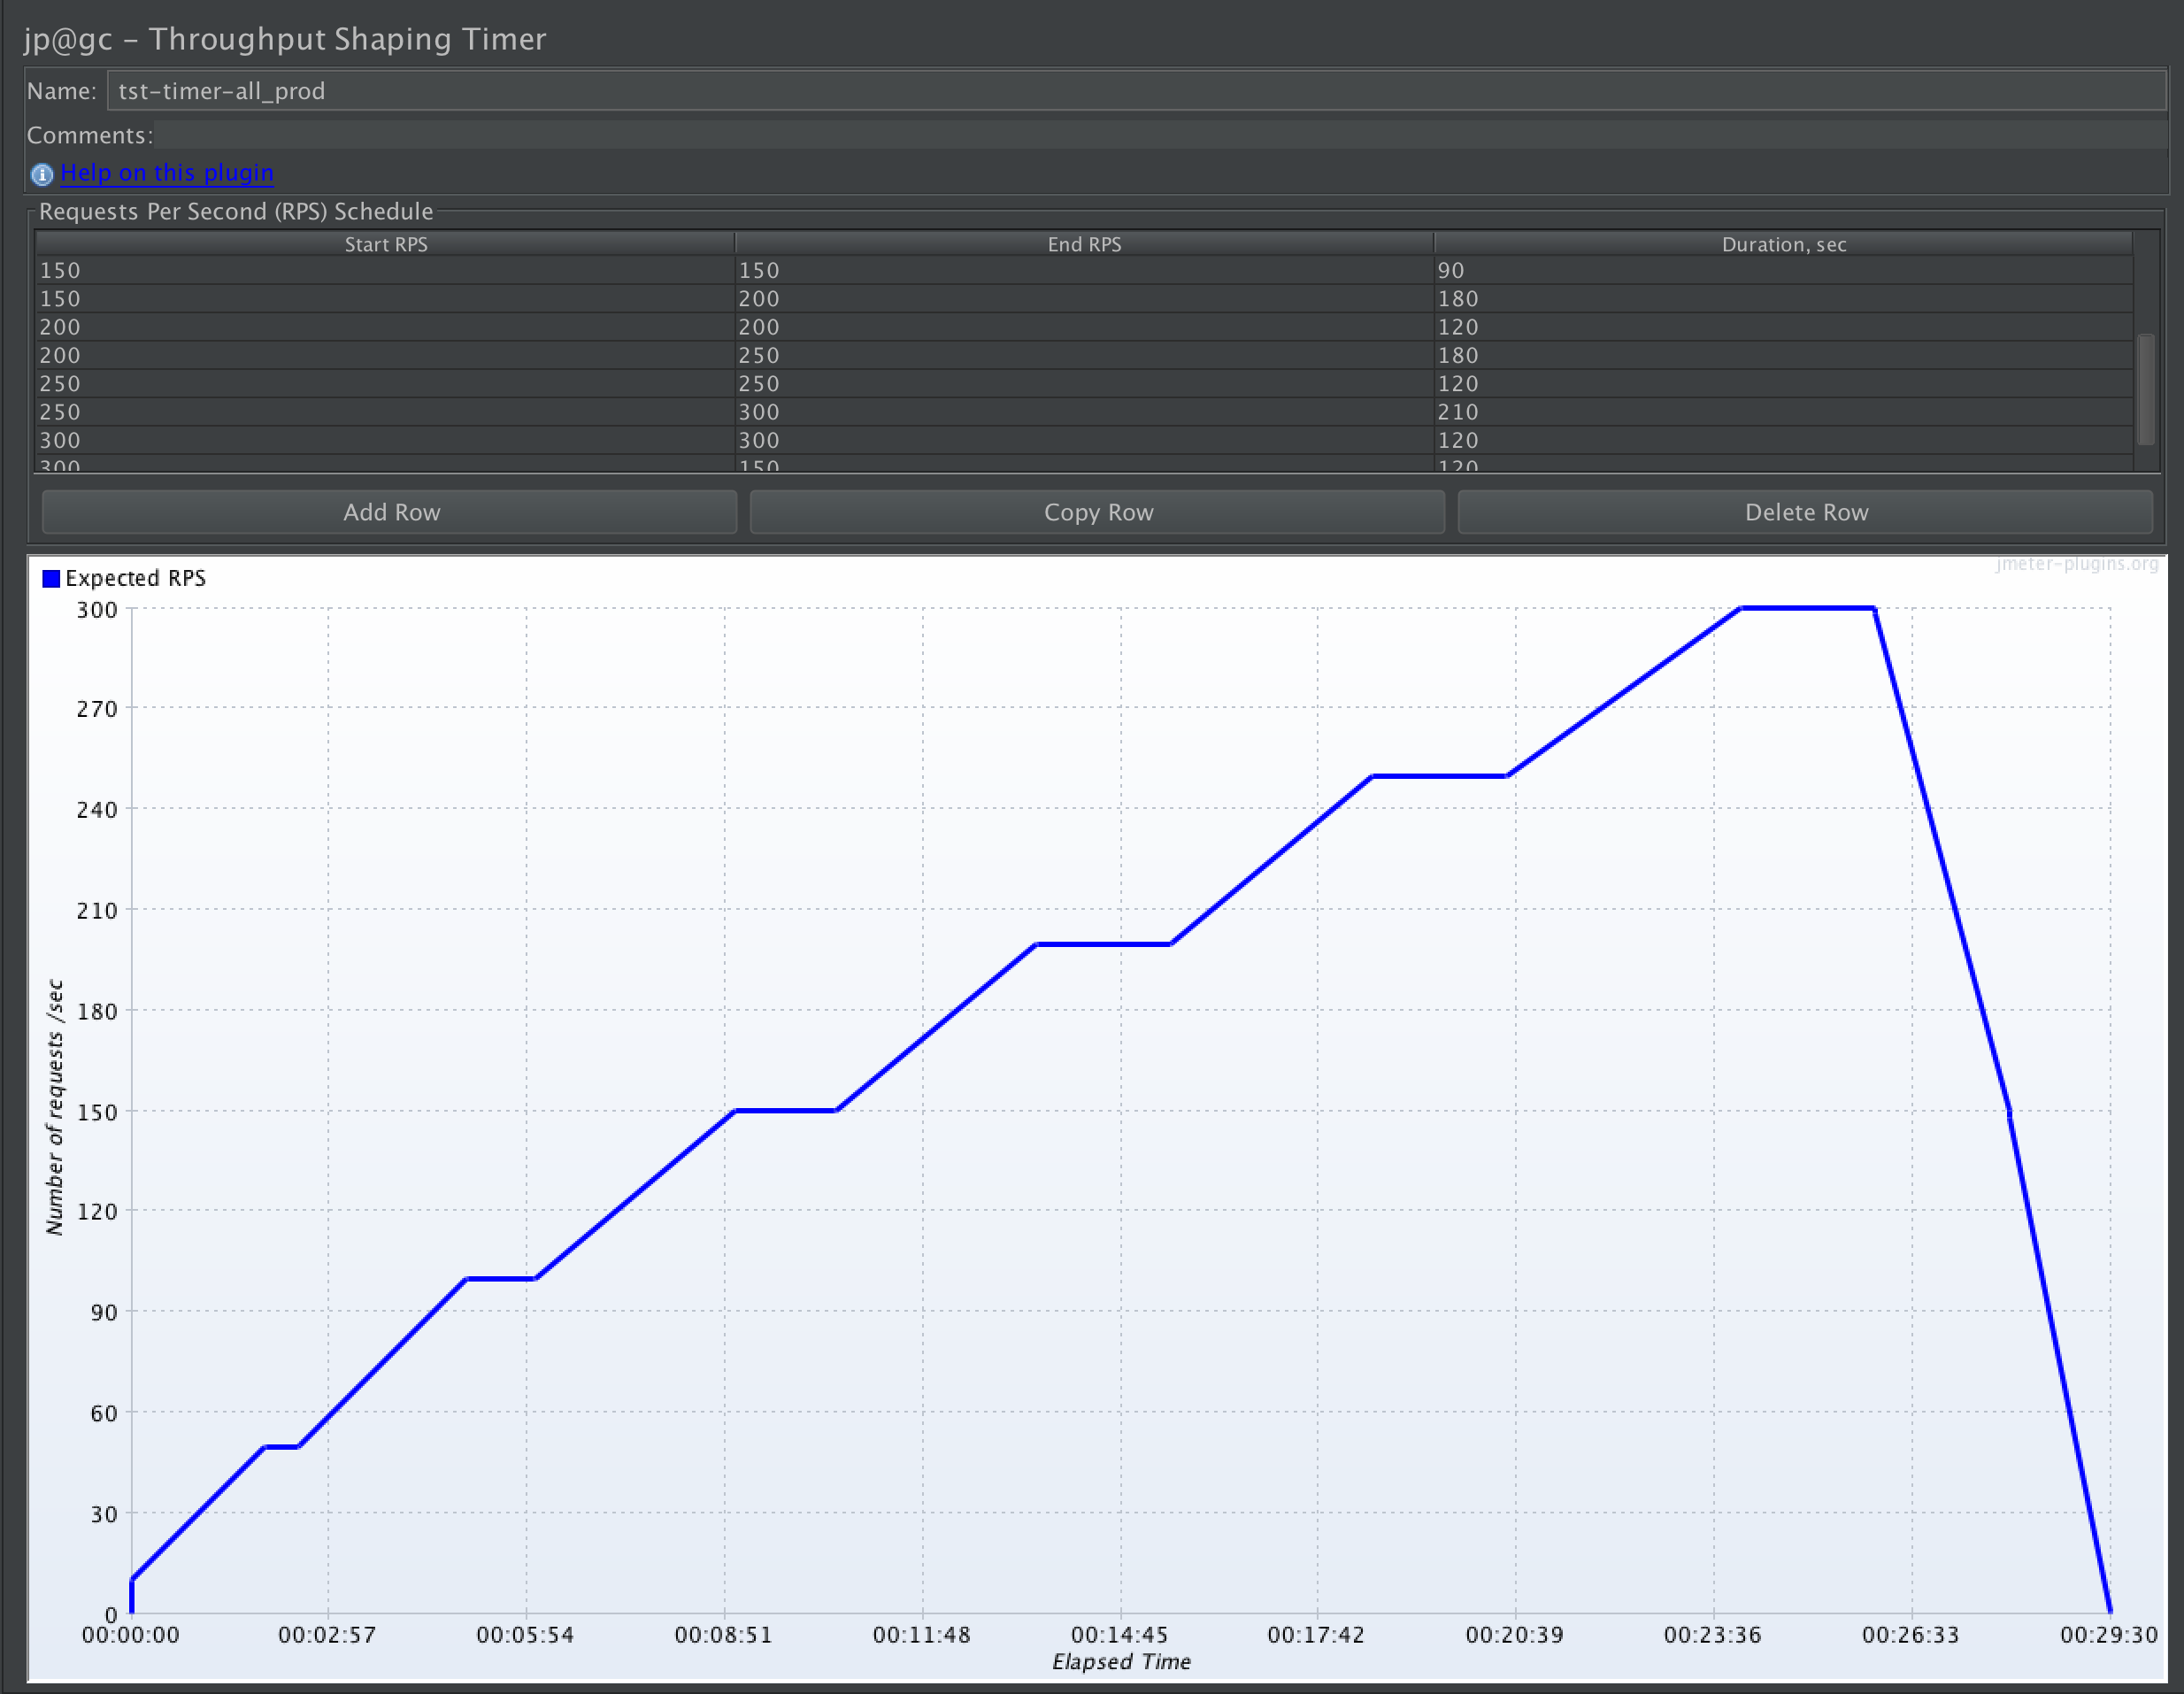
\includegraphics[width=0.8\textwidth]{results/work_load/test_prod_throughtput_shaping_timer.png}
    \caption{\acrshort{wdias} load testing throughput shaping timer \acrshort{rps} configurations}
    \label{fi:test_prod_throughtput_shaping_timer}
\end{figure}

\cref{fi:test_prod_throughtput_shaping_timer} shows the throughput shaping timer configurations use while load testing. The configurations as similar to the load test plan described in \cref{se:test_plan}. To get the maximum peak of 18,000 request per minutes, which is equivalent to 300 \acrshort{rps} is setup according the the figure.

%%%%%%%%%%%%%%%%%%%%%%%%%%%%%%%%%%%%%%%%%%%%%%%%%%%%%%%%%%%%%%%%%%%%%%%%%%%%%%%%
The test plans mentioned in \cref{se:test_plan} are implemented via the  JMeter. The following list shows the all the test cases used for the performance testing:

\begin{itemize}
    \item User-defined variables
    \item Setup thread group
    \item Create timeseries thread group
    \item Create extensions thread group
    \item Load test timeseries concurrency thread group
    \item Load test timeseries concurrency thread group
    \item Test flow thread group
\end{itemize}

The first step of the plan consists of setting up the timeseries metadata. At the same time, it creates the timeseries entry in the \acrshort{wdias} system as well as shown in the following list of test steps and configurations.

\begin{itemize}
    \item HTTP request defaults
    \item HTTP header manager
    \item Timeseries metadata CSV
    \item Create timeseries
    \item Get timeseries
    \item Query timeseries
\end{itemize}

By creating the timeseries before help to reduce the overhead during the performance testing, and cause to more accurate \acrshort{rps} at the run time.
Otherwise,  JMeter needs to allocate another set of threads for timeseries creation. Since the test cases insert data again set of timeseries, most of the time it about retrieving the timeseries metadata, rather than creating new timeseries in the \acrshort{wdias} system.

The following list shows the test steps of  JMeter while performing the load testing and the configurations.

\begin{itemize}
    \item HTTP Request Defaults
    \item HTTP Header Manager
    \item Timeseries Metadata CSV
    \item If Scalar or Vector
        \begin{itemize}
            \item Insert Timeseries
        \end{itemize}
    \item If a Grid
    \begin{itemize}
        \item Insert Grid Timeseries
    \end{itemize}
    \item Wait for extensions timeseries
    \item Interest Area preprocessor
    \item Query If Scalar Or Vector
    \item Retrieve If Scalar or Vector
        \begin{itemize}
            \item Retrieve Timeseries
        \end{itemize}
    \item Retrieve If a Grid
    \begin{itemize}
        \item Retrieve Grid Timeseries
    \end{itemize}
    \item Increment date
    \item Throughput shaping timer prod
\end{itemize}

As mentioned in \cref{se:test_plan}\hl{, we planned to perform another test scenario on the query timeseries module. During this test scenario, we use the following test steps to cover most of the timeseries metadata search queries and Geo queries which are defined in the} \cref{se:query}.

\begin{itemize}
    \item HTTP Request Defaults
    \item HTTP Header Manager
    \item Locations CSV
    \item Interest Area preprocessor
    \begin{itemize}
        \item /Location: * → Locations
    	\item /Location: Area → Locations
    	\item /Parameter: Location → Parameters
    	\item /Parameter: Locations → Parameters
    	\item /Timeseries: Location → Timeseries
    	\item /Timeseries: Locations → Timeseries
    	\item /Timeseries: Locations, Parameter → Timeseries
    	\item /Timeseries: Area → Timeseries
    	\item /Timeseries: Area, Parameter → Timeseries
    	\item /Timeseries: *, Parameter → Timeseries
    	\item /Timeseries: * → Timeseries
	\end{itemize}
\end{itemize}

\dbc{Top of Fig. 4.2 useless as it's black. Anyway, this figure isn't needed}
\gkc{Since we described about throughput shaping timer graph in \ref{subse:closed_vs_open_workload}, better to include it here. It include the details on RPS and how it's increasing over time. Will remove the black part. Also move this paragraph to the \cref{subse:closed_vs_open_workload}}

With the above  JMeter test case setup, it needs to enable each test case separately and before running via the command line in the server. To do it in a much efficient way, a scripting tool has implemented, and accessible with the codebase \cite{KarunarathneWdias-performance-test/TEST_PLAN.md:Plan} as \emph{test-dev}.

\begin{lstlisting}[language=sh, caption=Performance Test Help]
-h | --help: Usage
  test-dev enable <MODULE>
    - MODULE: import(i) | export(e) | extension(x) | all(a)

  test-dev run <REQ_SIZE>
    First need to enable module that need to be run
    - REQ_SIZE: 24(1) | 288(2) | 1440(3)
    NOTE: Modify test.conf as necessary
    e.g.
    test-dev run 24
    or
    test-dev run 1

  test-dev once <REQ_SIZE> <SEARCH_PHASE>
    This will enable the test case first. Then run the test case, and at the end disable and exit.
    - SEARCH_PHASE: Thread Group level name that matches
    e.g.
    test-dev once 24 CreateExtensions
    or
    test-dev once 1 CreateExtensions

  test-dev disable <MODULE>
    - MODULE: import(i) | export(e) | extension(x) | all(a)
\end{lstlisting}

As per the usage description of test-dev, it has the features of enabling a test case, disable a test case, and run the test case while enabled.
Another wrapper was implemented around the test-dev as \emph{test-plan.sh} which is also available with the codebase \cite{KarunarathneWdias-performance-test/TEST_PLAN.md:Plan}.

\begin{lstlisting}[language=sh, caption=Test Plan Help]
-h | --help: Usage
    <ROOT_DIR> <COMMAND> <REQ_SIZE>
    - COMMAND: setup | import | create_extension | extension | export | all | query
    - REQ_SIZE (optional): 24(1) | 288(2) | 1044(3)
  NOTE: Modify test.conf as necessary
  e.g.
  test_plan.sh ~/wdias/wdias-performance-test run 2
  - Run all the steps in order of setup, import, create_extension, extension, export, all, query
  test_plan.sh ~/wdias/wdias-performance-test run
  - Run all steps for all REQ_SIZE

  test_plan.sh ~/wdias/wdias-performance-test setup
  test_plan.sh ~/wdias/wdias-performance-test import 24
  test_plan.sh ~/wdias/wdias-performance-test all 24

  Distributed Mode
  SERVER_IPS=<IP1,IP2...> test_plan.sh ~/wdias/wdias-performance-test run
\end{lstlisting}

It allows running a particular test plan which is described in \cref{se:test_plan}. Also possible to run all the test plans in order with given \emph{REQ\_SIZE} or for all the \emph{REQ\_SIZE}.

\subsubsection{JMeter performance tuning}
\begin{itemize}
    \item Use CSV files rather than random number generation
    \item Use JSR223 scripts with Groovy for data processing for test cases
    \item Using Throughput Shaping Timer to get more accurate \acrshort{rps}
\end{itemize}


%%%%%%%%%%%%%%%%%%%%%%%%%%%%%%%%%%%%%%%%%%%%%%%%%%%%%%%%%%%%%%%%%%%%%%%%%%%%%%%%
\subsection{\hl{Test System Setup}}
\label{subse:test_sys_config}
As described in the \cref{se:microservice}, the \acrshort{wdias} is mainly focused on microservice architecture and implemented on top of Kubernetes. \acrfull{k8s} is an open-source system which is capable of automating deployment, scaling, and management of containerized applications. For the performance study uses \acrfull{eks}. There are many \acrshort{k8s} solutions available such as GCP, Azure, and Digital Ocean on the cloud.

A detailed description of setting up the \acrshort{eks} available as \cite{KarunarathneWdias/Amazon_EKS.md:EKS} within the main repository of the \acrshort{wdias}.
\acrshort{k8s} is a planet scaling tool \cite{LinuxFoundationProduction-GradeKubernetes}, and users can tweak the configuration to run the \acrshort{wdias} as per the required level of load on the system. During the performance test of the \acrshort{wdias}, it uses a maximum of 300 \acrshort{rps} with providing to the system with increasing load, and monitor the auto scalability of the system with measuring other performance parameters mentioned in \cref{tab:aws_eks_nodes}.

\begin{table}[ht]
\centering
\caption{\acrshort{eks} nodes}
\footnotesize
\begin{tabular}{|l|c|c|c|c|l|}
\hline
\textbf{Node Label} & \textbf{vCPU} & \textbf{RAM (GB)} & \textbf{Storage (GB)} & \textbf{Quantity} & \textbf{EC2 Name} \\ \hline
core & 16 & 32 & 15 & 1 & c5.4xlarge \\ \hline
grid & 8 & 16 & 25 & 1 & c5.2xlarge \\ \hline
scalar & 8 & 16 & 20 & 1 & c5.2xlarge \\ \hline
test & 4 & 10.5 & 5 & 1 & c5n.xlarge \\ \hline
\end{tabular}
\label{tab:aws_eks_nodes}
\end{table}
\dbc{Center table on page}
\gkc{FIXED}

The \acrshort{wdias} uses Helm \cite{CNCFHelmDocs} which is a package manager for \acrshort{k8s}. Each microservice within the system deploys and maintains as a helm chart, and the Helm Charts \cite{KarunarathneWdias-helm-charts:Deployments} can be found within the codebase. For the databases, it uses the official helm charts.


%%%%%%%%%%%%%%%%%%%%%%%%%%%%%%%%%%%%%%%%%%%%%%%%%%%%%%%%%%%%%%%%%%%%%%%%%%%%%%%%
\subsection{Performance Tuning}
\label{se:performance_tuning}
To get better performance using the available resources, it is possible to schedule each microservice into a predefined set of nodes. There are few ways to do in the \acrshort{k8s};
\begin{itemize}
    \item \emph{nodeSelector} -- Hard rules match for node schedule. If not match, pods will not schedule.
    \item \emph{node Affinity and Anti-Affinity} -- Soft rules for node schedule. Based on the rules, pods will schedule on the most appropriate node.
    \item \emph{Taints and Tolerations} -- Opposite of nodeSelector, repel mismatching pods away from the nodes.
\end{itemize}

\begin{figure}[htp]
    \centering
    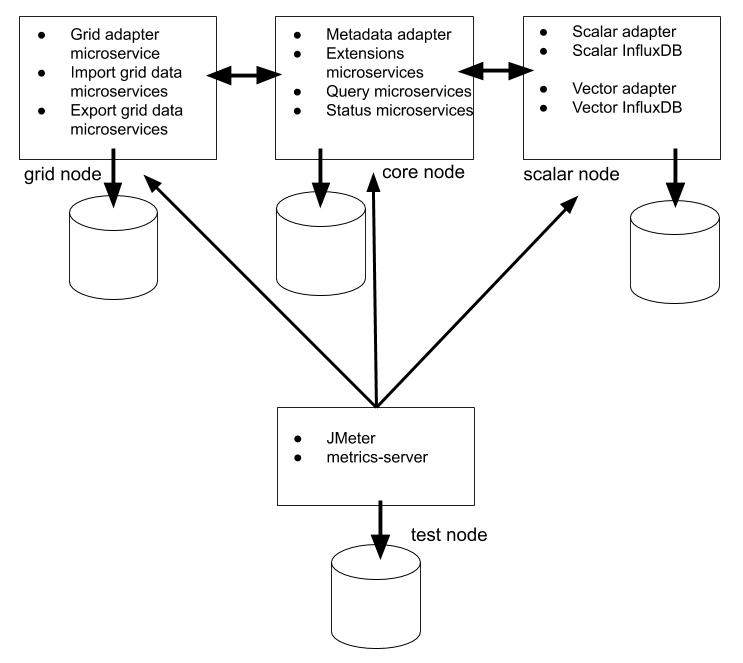
\includegraphics[width=0.75\textwidth]{results/work_load/eks_node_setup.jpg}
    \caption{\acrfull{eks} node setup}
    \label{fi:eks_node_setup}
\end{figure}

Users can use one of the above features to fine-tune the \acrshort{wdias} to perform better. For the moment, \acrshort{wdias} helm charts use node Affinity to use the same charts within local setup with one node and work the same charts on a \acrshort{k8s} cluster with multiple nodes. Pods are assigned to the nodes \cref{tab:aws_eks_nodes} based on the node label as below;
\begin{itemize}
    \item \emph{core} -- metadata, extensions, query, status and extension services
    \item \emph{grid} -- grid adapter, import and export grid data
    \item \emph{scalar} -- scalar and vector adapters, import and export of same data types
    \item \emph{test} --  JMeter and metric server
\end{itemize}
\cref{fi:eks_node_setup} shows the overview of the show the nodes are setup and each microservices are assigned to each node, the connectivity of the nodes, and the data interactions via the arrows.
The databases used for data consistency and performance in storage optimization with search capabilities. But because of that, it only possible to run one instance of those. In the \acrshort{wdias}, the MySQL and MongoDB are not getting higher load as adapter databases such as InfluxDB for scalar and vector data types, and netCDF for the grid data type. To keep up with the pace, those microservice pods are assigned to dedicated nodes to increase the performance of inter-service communication.
